\documentclass[a4paper,14pt,oneside,final]{extarticle}
\usepackage[top=2cm, bottom=2cm, left=3cm, right=1cm]{geometry}
\usepackage{scrextend}

\usepackage[T2A,T1]{fontenc}
\usepackage[ukrainian,russian,english]{babel}
\usepackage{tempora}
\usepackage{fontspec}
\setmainfont{tempora}

% Зачем: Отключает использование изменяемых межсловных пробелов.
% Почему: Так не принято делать в текстах на русском языке.
\frenchspacing

\usepackage{indentfirst}
\setlength{\parindent}{1.25cm}
\renewcommand{\baselinestretch}{1.5}

% Header
\usepackage{fancyhdr}
\pagestyle{fancy}
\fancyhead{}
\fancyfoot{}
\fancyhead[R]{\small \selectfont \thepage}
\renewcommand{\headrulewidth}{0pt}

% Captions
\usepackage{chngcntr}
\counterwithin{figure}{section}
\counterwithin{table}{section}
\usepackage[tableposition=top]{caption}
\usepackage{subcaption}
\DeclareCaptionLabelFormat{gostfigure}{Рисунок #2}
\DeclareCaptionLabelFormat{gosttable}{Таблиця #2}
\DeclareCaptionLabelSeparator{gost}{~---~}
\captionsetup{labelsep=gost}
\captionsetup[figure]{labelformat=gostfigure}
\captionsetup[table]{labelformat=gosttable}
\renewcommand{\thesubfigure}{\asbuk{subfigure}}

% Sections
\usepackage[explicit]{titlesec}
\newcommand{\sectionbreak}{\clearpage}

\titleformat{\section}
  {\centering}{\thesection \quad}{0pt}{\MakeUppercase{#1}}
\titleformat{\subsection}[block]
  {\bfseries}{\thesubsection \quad #1}{0cm}{}

\titlespacing{\section} {0cm}{0cm}{21pt}
\titlespacing{\subsection} {\parindent}{21pt}{0cm}
\titlespacing{\subsubsection} {\parindent}{0cm}{0cm}

% Lists
\usepackage{enumitem}
\renewcommand\labelitemi{--}
\setlist[itemize]{noitemsep, topsep=0pt, wide}
\setlist[enumerate]{noitemsep, topsep=0pt, wide, label=\arabic*}
\setlist[description]{labelsep=0pt, noitemsep, topsep=0pt, leftmargin=2\parindent, labelindent=\parindent, labelwidth=\parindent, font=\normalfont}

% Toc
\usepackage{tocloft}
\tocloftpagestyle{fancy}
\renewcommand{\cfttoctitlefont}{}
\setlength{\cftbeforesecskip}{0pt}
\renewcommand{\cftsecfont}{}
\renewcommand{\cftsecpagefont}{}
\renewcommand{\cftsecleader}{\cftdotfill{\cftdotsep}}

\usepackage{float}
\usepackage{pgfplots}
\usepackage{graphicx}
\usepackage{multirow}
\usepackage{amssymb,amsfonts,amsmath,amsthm}
\usepackage{csquotes}

\usepackage{listings}
\lstset{basicstyle=\footnotesize\ttfamily,breaklines=true}
\lstset{language=Matlab}

\usepackage[
	backend=biber,
	sorting=none,
	language=auto,
	autolang=other
]{biblatex}
\DeclareFieldFormat{labelnumberwidth}{#1}

\lstdefinelanguage{Python}{
  keywords={and, break, class, continue, def, yield, del, elif, else, except, exec, finally, for, from, global, if, import, in, lambda, not, or, pass, print, raise, return, try, while, assert, with},
  keywordstyle=\color{NavyBlue}\bfseries,
  ndkeywords={True, False},
  ndkeywordstyle=\color{BurntOrange}\bfseries,
  emph={as},
  emphstyle={\color{OrangeRed}},
  identifierstyle=\color{black},
  sensitive=true,
  commentstyle=\color{gray}\ttfamily,
  comment=[l]{\#},
  morecomment=[s]{/*}{*/},
  stringstyle=\color{ForestGreen}\ttfamily,
  morestring=[b]',
  morestring=[s]{"""*}{*"""},
}


\newcommand{\tasknumber}{1} % first

\documentclass[a4paper,14pt,oneside,final]{extarticle}
\usepackage[top=2cm, bottom=2cm, left=3cm, right=1cm]{geometry}
\usepackage{scrextend}

\usepackage[T2A,T1]{fontenc}
\usepackage[ukrainian,russian,english]{babel}
\usepackage{tempora}
\usepackage{fontspec}
\setmainfont{tempora}

% Зачем: Отключает использование изменяемых межсловных пробелов.
% Почему: Так не принято делать в текстах на русском языке.
\frenchspacing

\usepackage{indentfirst}
\setlength{\parindent}{1.25cm}
\renewcommand{\baselinestretch}{1.5}

% Header
\usepackage{fancyhdr}
\pagestyle{fancy}
\fancyhead{}
\fancyfoot{}
\fancyhead[R]{\small \selectfont \thepage}
\renewcommand{\headrulewidth}{0pt}

% Captions
\usepackage{chngcntr}
\counterwithin{figure}{section}
\counterwithin{table}{section}
\usepackage[tableposition=top]{caption}
\usepackage{subcaption}
\DeclareCaptionLabelFormat{gostfigure}{Рисунок #2}
\DeclareCaptionLabelFormat{gosttable}{Таблиця #2}
\DeclareCaptionLabelSeparator{gost}{~---~}
\captionsetup{labelsep=gost}
\captionsetup[figure]{labelformat=gostfigure}
\captionsetup[table]{labelformat=gosttable}
\renewcommand{\thesubfigure}{\asbuk{subfigure}}

% Sections
\usepackage[explicit]{titlesec}
\newcommand{\sectionbreak}{\clearpage}

\titleformat{\section}
  {\centering}{\thesection \quad}{0pt}{\MakeUppercase{#1}}
\titleformat{\subsection}[block]
  {\bfseries}{\thesubsection \quad #1}{0cm}{}

\titlespacing{\section} {0cm}{0cm}{21pt}
\titlespacing{\subsection} {\parindent}{21pt}{0cm}
\titlespacing{\subsubsection} {\parindent}{0cm}{0cm}

% Lists
\usepackage{enumitem}
\renewcommand\labelitemi{--}
\setlist[itemize]{noitemsep, topsep=0pt, wide}
\setlist[enumerate]{noitemsep, topsep=0pt, wide, label=\arabic*}
\setlist[description]{labelsep=0pt, noitemsep, topsep=0pt, leftmargin=2\parindent, labelindent=\parindent, labelwidth=\parindent, font=\normalfont}

% Toc
\usepackage{tocloft}
\tocloftpagestyle{fancy}
\renewcommand{\cfttoctitlefont}{}
\setlength{\cftbeforesecskip}{0pt}
\renewcommand{\cftsecfont}{}
\renewcommand{\cftsecpagefont}{}
\renewcommand{\cftsecleader}{\cftdotfill{\cftdotsep}}

\newcommand{\khpistudentgroup}{2.КН201н.8а}
\newcommand{\khpistudentname}{Чепурний~А.~С.}

\newcommand{\khpidepartment}{Програмна інженерія та інформаційні технології управління}
\newcommand{\khpititlewhat}{
	Розрахунково-графічне завдання №\tasknumber \\
	з предмету <<Основи проектування інтелектуальних систем>>
}
\newcommand{\khpititlewho}{
	Виконав: \\
	\hspace*{\parindent} ст. групи \khpistudentgroup \\
	\hspace*{\parindent} \khpistudentname \\
	Перевірила: \\
	\hspace*{\parindent} ст. в. каф. ПІІТУ \\
	\hspace*{\parindent} Єршова~С.~І. \\
}


\graphicspath{{figures/}}

\begin{document}
\Ukrainian

\begin{titlepage}

\begin{center}
	МІНІСТЕРСТВО ОСВІТИ І НАУКИ УКРАЇНИ \\
	НАЦІОНАЛЬНИЙ ТЕХНІЧНИЙ УНІВЕРСИТЕТ \\
	«ХАРКІВСЬКИЙ ПОЛІТЕХНІЧНИЙ ІНСТИТУТ» \\[0.5cm]
	Кафедра <<\khpidepartment>> \\
\end{center}

\vspace{6cm}

\begin{center}
	\khpititlewhat
\end{center}

\vspace{3cm}

\begin{addmargin}[10cm]{0cm}
	\khpititlewho
\end{addmargin}

\vspace{\fill}

\begin{center}
	Харків \the\year
\end{center}

\end{titlepage}

\addtocounter{page}{1}

\subsection{Семантична мережа}
\textit{Петрик п'є молоко зі стакану.}

На рисунку~\ref{fig:semantic_int}зображено  інтенсіональну семантичну мережу для даної фрази.

\begin{figure}[H]
    \centering
        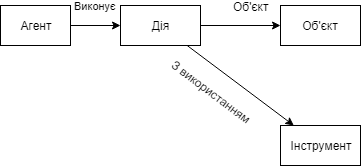
\includegraphics{semantic_int}
    \caption{Інтенсіональна семантична мережа}
    \label{fig:semantic_int}
\end{figure}

На рисунку~\ref{fig:semantic_ext} зображено екстенсіональну семантичну мережа для даної фрази.

\begin{figure}[H]
    \centering
        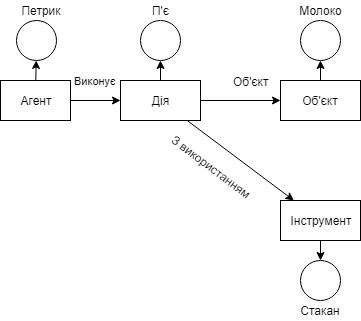
\includegraphics[width=0.7\linewidth]{semantic_ext}
    \caption{Екстенсіональна семантична мережа}
    \label{fig:semantic_ext}
\end{figure}

\subsection{Семантична мережа з десигнатом}
\textit{Дитина п'є молоко зі стакану.}

На рисунку~\ref{fig:semantic_ext_ds} зображено семантичну мережу з десигнатом для даної фрази.

\begin{figure}[H]
    \centering
        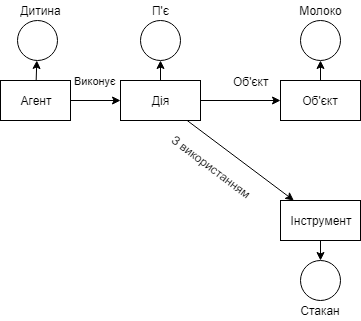
\includegraphics[width=0.7\linewidth]{semantic_ext_ds}
    \caption{Семантична мережа з десигнатом}
    \label{fig:semantic_ext_ds}
\end{figure}

Десигнатом, у даному випадку, є <<Дитина>>. 
Це умовлено тим, що даний агент має унікальне внутрісистемне ім'я, але про нього немає повної інформації.

У виді фрейму дана мережа представлена у таблиці~\ref{tab:semantic_ext_ds}.

\begin{table}[H]
  \begin{tabular}{|c|c|}
    \hline
    Агент & Дитина \\ \hline
    Дія & П'є \\ \hline
    Об'єкт & Молоко \\ \hline
    Інструмент & Стакан \\ \hline
  \end{tabular}
  \caption{Семантична мережа з десигнатом}
  \label{tab:semantic_ext_ds}
\end{table}

\subsection{Концептуальний граф}
\textit{Мати думає, що Петрик п'є напій з молока та чаю.}

На рисунку~\ref{fig:semantic_con} зображено концептуальний граф для даної фрази.

\begin{figure}[H]
    \centering
        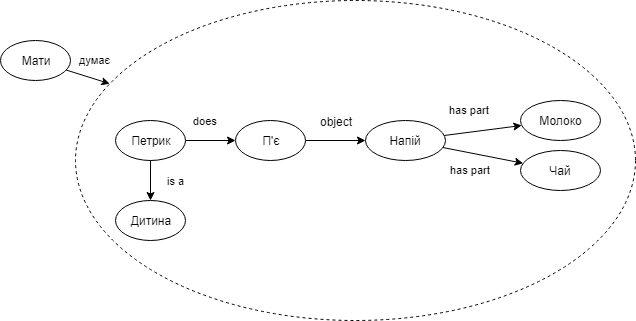
\includegraphics[width=\linewidth]{semantic_con}
    \caption{Концептуальний граф}
    \label{fig:semantic_con}
\end{figure}

\subsection{Граф Раст'є}
\textit{Дитина п'є молоко зі стакану, щоб набути здоров'я.}

На рисунку~\ref{fig:semantic_ras} зображено граф Раст'є для даної фрази.

\begin{figure}[H]
    \centering
        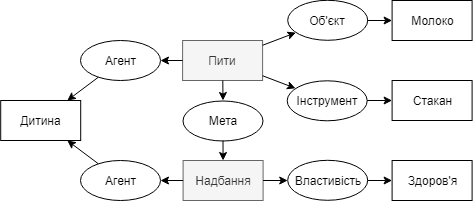
\includegraphics[width=\linewidth]{semantic_ras}
    \caption{Граф Раст'є}
    \label{fig:semantic_ras}
\end{figure}

\subsection{Реляційний граф}
\textit{Петрик п'є напій з молока та чаю.}

На рисунку~\ref{fig:semantic_rel} зображено реляційний граф для даної фрази.

\begin{figure}[H]
    \centering
        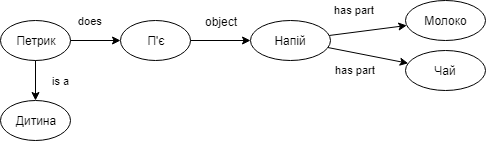
\includegraphics[width=\linewidth]{semantic_rel}
    \caption{Реляційний граф}
    \label{fig:semantic_rel}
\end{figure}

\subsection*{Висновки}
В данній роботі були розглянуті та побудовані такі види семантичних мереж, як інтенсіональна семантична мережа, екстенсіональна семантична мережа, мережа з десигнатом, концептуальний граф, граф Раст'є та реляційний граф.

Семантичні мережі використовуються для відображення зв'язків між об'єктами предметної області.
Граф Раст'є використовується для представлення подій.
Граф Раст'є дозволяє уникнути вкладеності графів.

Семантична мережа з бінарними відношеннями назвається концептуальним графом, та використовується для систематизації концептів предметної області та зв’язків між ними.

Реляційний граф використовується для класифікації та систематизації об’єктів предметної області а також для відображення зв’язків між ними.

\end{document}
